% Created 2020-04-24 Fri 11:49
% Intended LaTeX compiler: pdflatex
\documentclass[11pt]{article}
\usepackage[utf8]{inputenc}
\usepackage[T1]{fontenc}
\usepackage{graphicx}
\usepackage{grffile}
\usepackage{longtable}
\usepackage{wrapfig}
\usepackage{rotating}
\usepackage[normalem]{ulem}
\usepackage{amsmath}
\usepackage{textcomp}
\usepackage{amssymb}
\usepackage{capt-of}
\usepackage{hyperref}
\author{Mikael Svahnberg}
\date{\today}
\title{Example System: BurgerOrderer}
\hypersetup{
 pdfauthor={Mikael Svahnberg},
 pdftitle={Example System: BurgerOrderer},
 pdfkeywords={},
 pdfsubject={},
 pdfcreator={Emacs 26.3 (Org mode 9.1.9)}, 
 pdflang={English}}
\begin{document}

\maketitle
\tableofcontents

\section{Use Case: Order Food}
\label{sec:org08000b8}
Use case: Order Food
Actors: Customer
Description: A customer arrives at the BurgerOrderer, selects a meal, configures their hamburger, and orders it.
Related Use cases: Pay for Order

Main Course of Events
\begin{center}
\begin{tabular}{ll}
Actor & System\\
\hline
1. Customer arrives at BurgerOrderer and starts a new order & \\
 & 2. System presents options\\
 & [just one burger, full meal, dessert, drink]\\
3. Customer selects "full meal" & \\
 & 4. System presents available meals\\
5. Customer selects a meal & \\
 & 6. System adds the selected meal to order and\\
 & presents configuration options\\
7. Customer selects "no onions" & \\
 & 8. System adds "no onions" to the order\\
9. Customer selects "more bacon!" & \\
 & 10. System adds "more bacon!" to the order\\
11. Customer confirms order & \\
 & 12. System initiates use case \uline{pay for order} .\\
 & 13. System places burger order to the kitchen\\
 & and prints a receipt.\\
\hline
\end{tabular}
\end{center}
\section{System Sequence Diagram}
\label{sec:org7c97468}
\begin{verbatim}
actor ":Customer" as customer
participant ":BurgerOrderer" as sys

customer -> sys : startNewOrder()
sys --> customer : present options [one burger, meal, dessert, drink]
customer -> sys : select("meal")
sys --> customer : present meals
customer -> sys : selectMeal("Max")
sys --> customer : present configuration options
customer -> sys : selectOption("no onions")
customer -> sys : selectOption("moar bacon!")
customer -> sys : confirmOrder()


\end{verbatim}

\begin{center}
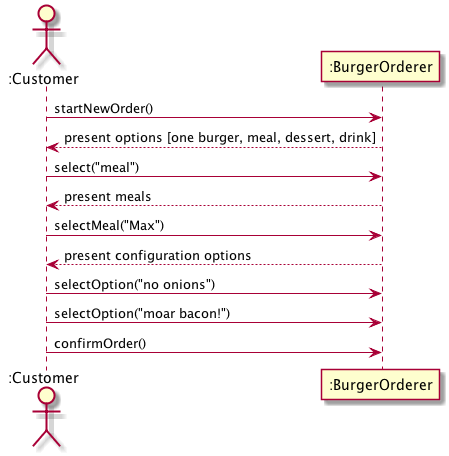
\includegraphics[width=.9\linewidth]{202004-bo-ssd.png}
\end{center}

\section{Interaction Diagrams (Sequence Diagrams)}
\label{sec:org20df242}
\subsection{startNewOrder()}
\label{sec:orgfd2464f}
\begin{verbatim}
participant ":BurgerOrderer" as sys

[-> sys : startNewOrder()
activate sys
' ---------- How the system intents to solve this system call is described below ----------
sys --> ":Order" : create()
sys -> ":OrderTypeManager" : getOrderTypes()
[<-- sys : return types of orders
' ---------- end ----------
deactivate sys
\end{verbatim}

\begin{center}
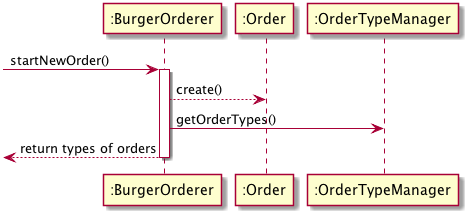
\includegraphics[width=.9\linewidth]{202004-bo-startNew.png}
\end{center}

\subsection{selectOrderType()}
\label{sec:orgfc5da88}
\begin{verbatim}
participant ":BurgerOrderer" as sys

[-> sys : selectOrderType(theOrderTypeName)
activate sys
' ---------- How the system intents to solve this system call is described below ----------
sys -> ":OrderTypeManager" : getOrderType(theOrderTypeName)
activate ":OrderTypeManager"
":OrderTypeManager" --> "ot:OrderType" : create()
":OrderTypeManager" --> sys : return ot
deactivate ":OrderTypeManager"

sys -> "ot:OrderType" : getAvailableItems()
activate "ot:OrderType"
deactivate "ot:OrderType"

[<-- sys : return available items
' ---------- end ----------
deactivate sys
\end{verbatim}

\begin{center}
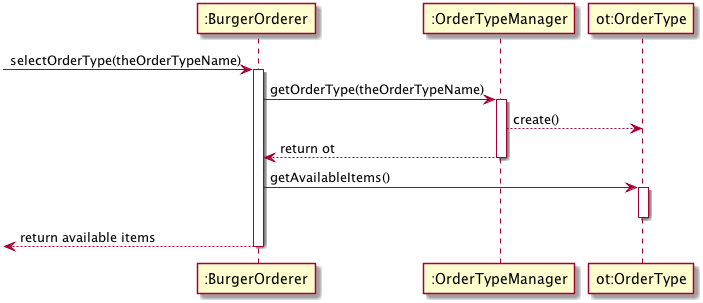
\includegraphics[width=.9\linewidth]{202004-bo-selectOT.png}
\end{center}

\subsection{selectItem("MaxMeal")}
\label{sec:org95024bb}
\begin{verbatim}
participant ":BurgerOrderer" as sys

[-> sys : selectItem(itemName)
activate sys
' ---------- How the system intents to solve this system call is described below ----------
sys -> "ot:OrderType" : selectItem(itemName)
activate "ot:OrderType"
"ot:OrderType" --> "theItem:Item" : create()
"ot:OrderType" --> sys : theItem
deactivate "ot:OrderType"
sys -> ":Order" : addItem(theItem)
activate ":Order"
deactivate ":Order"

sys -> "theItem:Item" : getOptions()
activate "theItem:Item"
deactivate "theItem:Item"
[<-- sys : return list of options
' ---------- end ----------
deactivate sys
\end{verbatim}

\begin{center}
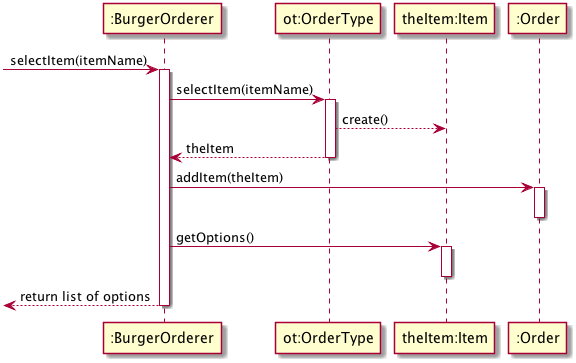
\includegraphics[width=.9\linewidth]{202004-bo-selectItem.png}
\end{center}
\subsection{selectOption("no onions")}
\label{sec:orgd8041bf}
\begin{verbatim}
participant ":BurgerOrderer" as sys

[-> sys : selectOption(optionName)
activate sys
' ---------- How the system intents to solve this system call is described below ----------
sys -> "theItem:Item" : selectOption(optionName)
activate "theItem:Item"
"theItem:Item" -> "theItem:Item" : op = getOption(optionName)
activate "theItem:Item"
deactivate "theItem:Item"

"theItem:Item" -> "op:ItemOption" : enable()
activate "op:ItemOption"
deactivate "op:ItemOption"

deactivate "theItem:Item"
' ---------- end ----------
deactivate sys
\end{verbatim}

\begin{center}
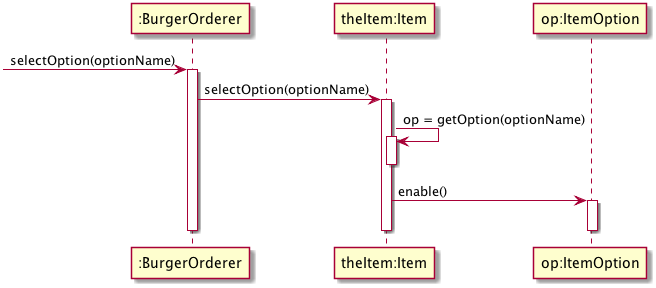
\includegraphics[width=.9\linewidth]{202004-bo-selectOption.png}
\end{center}

\subsection{selectOption("more bacon!")}
\label{sec:org607aff7}
\subsection{confirmOrder()}
\label{sec:org52dd479}
\begin{verbatim}
participant ":BurgerOrderer" as sys

[-> sys : confirmOrder()
activate sys
' ---------- How the system intents to solve this system call is described below ----------
sys -> ":Payment" : executePayment()
activate ":Payment"
deactivate ":Payment"

sys -> ":Order" : sendOrder()
activate ":Order"
":Order" -> ":KitchenController" : sendItems(items)
activate ":KitchenController"
deactivate ":KitchenController"
deactivate ":Order"

sys -> ":Order" : printReceipt()
activate ":Order"

loop for all Items in Order
":Order" -> ":ReceiptPrinter" : print(theItem)
activate ":ReceiptPrinter"
":ReceiptPrinter" -> "theItem:Item" : getName()
activate "theItem:Item"
deactivate "theItem:Item"
":ReceiptPrinter" -> "theItem:Item" : getEnabledOptionNames()
activate "theItem:Item"
loop for all options
"theItem:Item" -> "option:ItemOption" : isEnabled()
activate "option:ItemOption"
deactivate "option:ItemOption"

alt is Enabled
"theItem:Item" -> "option:ItemOption" : getName()
activate "option:ItemOption"
deactivate "option:ItemOption"
end alt

end loop
deactivate "theItem:Item"

deactivate ":ReceiptPrinter"
end loop
deactivate ":Order"

' ---------- end ----------
deactivate sys
\end{verbatim}

\begin{center}
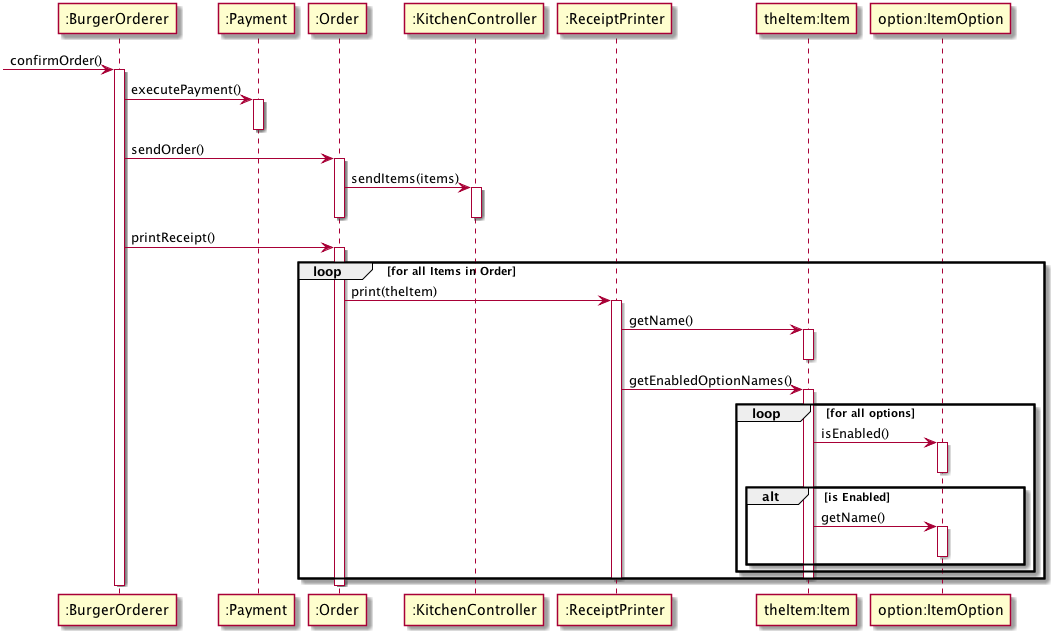
\includegraphics[width=.9\linewidth]{202004-bo-confirmorder.png}
\end{center}

\section{Class Diagram}
\label{sec:orgaa76282}
\begin{verbatim}
class BurgerOrderer {
+startNewOrder()
+selectOrderdType(string theOrderTypeName)
+selectItem(string itemName)
+selectOption(string optionName)
}

class Order {
 +addItem(Item theItem)
}

OrderTypeManager : +OrderType[] getOrderTypes()
OrderTypeManager : +OrderType* getOrderType(string theOrderTypeName)

abstract class OrderType <<abstract strategy>>
OrderType : +getAvailableItems()
OrderType : +selectItem(string itemName)
OrderType <|-- MealOrderType
OrderType <|-- PlainBurgerOrderType
OrderType <|-- DessertOrderType

Item : +string[] getOptionNames() ' TODO: rename getOptions() in seq-diagr.
Item : +selectOption(string optionName)
Item : +ItemOption* getOption(string optionName)

ItemOption : enable()

BurgerOrderer - Order
BurgerOrderer -- OrderTypeManager
BurgerOrderer --- OrderType
BurgerOrderer -- Item : >

OrderTypeManager -- "*" OrderType

Item -- "*" ItemOption

Order -- "*" Item

\end{verbatim}

\begin{center}
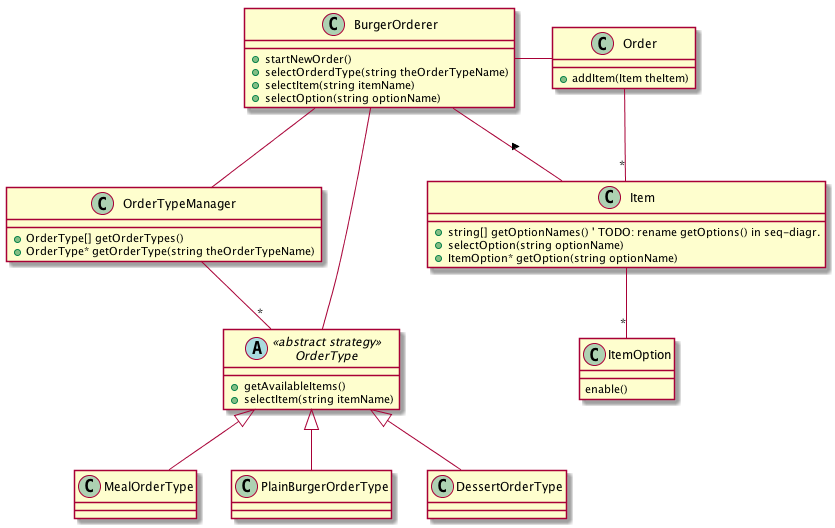
\includegraphics[width=.9\linewidth]{202004-classes.png}
\end{center}

\section{Entity Component System}
\label{sec:org594d5b3}
Ett förslag på hur man kan göra "OrderType" annorlunda, för att slippa en del problem om man vill sätta ihop nya ordertyper.
\subsection{Bakgrund: lös det med arv}
\label{sec:orgcca613c}
Hur man skulle behövt lösa kompositionen om man inte använt ECS utan vanliga arvshierarkier
\begin{verbatim}
OrderType <|-- Meal
OrderType <|-- PlainBurger
OrderType <|-- Dessert
OrderType <|-- Drink

PlainBurger <|-- BurgerWithDessert
Dessert <|-- BurgerWithDessert

BurgerWithDessert <|-- SameButWithDrinkToo
Drink <|-- SameButWithDrinkToo

\end{verbatim}

\begin{center}
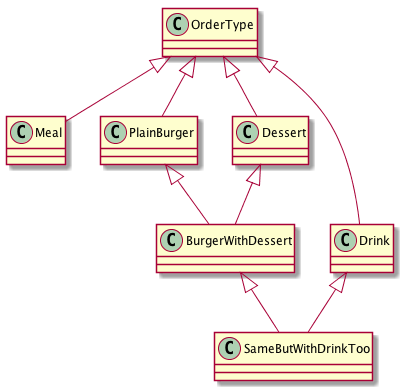
\includegraphics[width=.9\linewidth]{202004-ecs-inheritance.png}
\end{center}

\ldots{} Som synes så blir det nya (multipla) arv varje gång man vill skapa en ny ordertyp. Jobbigt, svårt med multipla arv, man måste koda om systemet varje gång man vill skapa en ny ordertyp.

\subsection{Alternaiv: Entity Component System}
\label{sec:org020b517}
\begin{verbatim}

class OrderType {
 +getAvailableItems()
 +selectItem(string itemName)
}

abstract class MealComponent
MealComponent <|-- PlainBurger
MealComponent <|-- Dessert
MealComponent <|-- Fries
MealComponent <|-- Drink

OrderType o-- "*" MealComponent

\end{verbatim}

\begin{center}
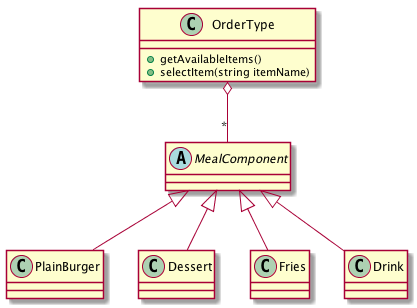
\includegraphics[width=.9\linewidth]{202004-ecs.png}
\end{center}

\begin{verbatim}
// Note: Here be dragons! Egregious pseudocode below...
class OrderType {
private:
 MealComponent** myComponents;
public:
 void create(string** componentNames) {
  for(c in componentNames) {
    myComponents.push(createNewMealComponent(c));
  }
}

 MealComponent* createNewMealComponent(string cName) {
   switch (cName) {
 case "Burger" : return new PlainBurger(); break;
 case "Dessert" : return new Dessert(); break;
}
}
}
\end{verbatim}

Slutsats: Lätt att kombinera ihop nya ordertyper -- vid runtime om så krävs.
\end{document}